\documentclass[11pt,a4paper]{article}

\usepackage[margin=2.5cm]{geometry}
\usepackage[T1]{fontenc}
\usepackage{lmodern}
\usepackage{microtype}
\usepackage{amsmath,amssymb}
\usepackage{booktabs}
\usepackage{graphicx}
\usepackage{float}
\usepackage{xcolor}
\usepackage{enumitem}
\usepackage{siunitx}
\usepackage{caption}
\usepackage{fancyhdr}
\usepackage{pgfplots}
\usepackage{tikz}
\usetikzlibrary{shapes.geometric,arrows.meta,positioning,calc}
\pgfplotsset{compat=1.17}
\usepackage[colorlinks=true,linkcolor=black,citecolor=blue!50!black,urlcolor=blue!50!black]{hyperref}

\captionsetup{font=small,labelfont=bf,skip=6pt}
\setlength{\parindent}{0pt}
\setlength{\parskip}{0.6em}
\renewcommand{\arraystretch}{1.2}

\pagestyle{fancy}
\fancyhf{}
\lhead{\small SunSync: Dual Axis Sun Tracking Solar Panel}
\rhead{\small ENGR1000J Project 2}
\cfoot{\small\thepage}
\renewcommand{\headrulewidth}{0.3pt}

\definecolor{accent}{HTML}{1F4E79}
\usepackage{titlesec}
\titleformat{\section}{\Large\bfseries\color{accent}}{\thesection}{0.6em}{}
\titleformat{\subsection}{\large\bfseries}{\thesubsection}{0.6em}{}

\begin{document}

% ---------- Title block ----------
\begin{center}
  {\Large\bfseries\color{accent} ENGR1000J Introduction to Engineering, Project 2 Lab Report\par}
  \vspace{0.8em}
  {\fontsize{24}{28}\selectfont\bfseries SunSync\par}
  \vspace{0.3em}
  {\Large A Dual Axis Sun Tracking Solar Panel\par}
  \vspace{1em}
  UM-SJTU Joint Institute, Shanghai Jiao Tong University\par
  Group 2 (team of four) \quad|\quad Original report: 1 December 2024
\end{center}

\vspace{0.5em}
\noindent\fbox{\parbox{\dimexpr\textwidth-2\fboxsep-2\fboxrule\relax}{\small
\textbf{About this edition.} This is a reorganised and rewritten version of the Group 2 lab report. Every observation in it comes from the original report and the project code. No new measurements were added. Wording that claimed more than the evidence supports has been corrected, and the main limitation (no measured comparison with a fixed panel) is stated openly in Sections~\ref{sec:results} and~\ref{sec:discussion}.}}

\vspace{1em}

% ---------- Abstract ----------
\begin{abstract}
\noindent
We built a prototype sun tracking solar panel that follows a light source on two axes. Four light dependent resistors (LDRs) mounted around the panel measure how light is distributed across it, and an Arduino microcontroller drives two servo motors to move the panel toward the brighter side until the readings balance. In two flashlight trials the panel followed the moving light and the output stayed stable, and the firmware drives each axis over a range of \ang{180}. A simple idealised model, in which the tracker always faces the light and a fixed horizontal panel does not, predicts that tracking collects $\pi/2\approx1.57$ times as much energy over a day. This ratio is a theoretical estimate. The prototype's energy output was not compared against a fixed panel in a quantitative test.
\end{abstract}

% ---------- 1 ----------
\section{Introduction}

The effects of climate change, such as rising temperatures, extreme weather and shifting ecosystems, are becoming more evident. The Intergovernmental Panel on Climate Change (IPCC) links these changes mainly to human activity, particularly the burning of fossil fuels, which releases greenhouse gases \cite{ipcc}. At the same time, global energy demand keeps growing as populations increase and developing countries industrialise. Coal, oil and natural gas are becoming harder to justify because of their environmental impact and limited supply.

Renewable energy, and solar power in particular, has gained attention because it is abundant, scalable and increasingly accessible. The best fixed solar panels reach an efficiency of around \SI{25}{\percent} \cite{cnet}. A fixed panel, however, cannot stay aligned with the sun as it moves from east to west, so it loses energy for much of the day.

A sun tracking panel addresses this by turning to face the light source. It can raise the energy collected without adding panels or land. This report describes the design, operation and testing of a small sun tracking prototype, and estimates how much better tracking could be compared with a fixed panel.

% ---------- 2 ----------
\section{Theoretical Background}

\subsection{Inspiration from nature}
Sunflowers show \emph{heliotropism}: their flower heads turn to follow the sun from east to west, keeping the head facing the light to support photosynthesis \cite{helio}. Our panel imitates this behaviour.

\subsection{Photovoltaic conversion and incidence angle}
A solar panel converts light to electricity through the photovoltaic effect: light absorbed in a semiconductor junction frees charge carriers, which produces a voltage and a current \cite{pv}. The power a panel receives depends on how directly the light strikes it. If $\theta$ is the angle between the sunlight and the panel surface and $S$ is the panel area, the effective collecting area is
\begin{equation}
  S_{\text{eff}} = S\sin\theta .
\end{equation}
The maximum occurs at $\theta=\ang{90}$, when the sunlight is perpendicular to the panel. Holding the panel perpendicular to the light therefore gives the greatest output.

\subsection{Two axis tracking}
Two servo motors make this possible. One rotates the panel horizontally to follow the sun from east to west. The other tilts the panel vertically to follow the sun's changing elevation through the day.

\subsection{Locating the light with LDRs}
A light dependent resistor (LDR), also called a photoresistor, is a passive component whose resistance drops as the light on it increases. One LDR sits at each of the four corners of the panel (top left, top right, bottom left and bottom right). When the panel faces the light squarely, all four read about the same. If one side is brighter, the LDRs on that side read as more illuminated, which tells the controller which way to turn.

% ---------- 3 ----------
\section{Theoretical Efficiency Gain}
\label{sec:theory}

\subsection{Idealised model}
The comparison below uses the same simplifying assumptions as the original report:
\begin{itemize}[nosep]
  \item The tracking panel always faces the light, so $\sin\theta=1$ throughout the day.
  \item The fixed panel lies flat, and the angle between the sunlight and its surface follows $\theta=\pi x$, where $x\in[0,1]$ is the fraction of the \num{12}-hour day that has passed.
\end{itemize}
Relative output is then proportional to $f(x)=1$ for the tracker and $g(x)=\sin(\pi x)$ for the fixed panel (Figure~\ref{fig:curves}). The ratio of the energy collected over the day is the ratio of the areas under the two curves:
\begin{equation}
  \frac{E_{\text{tracking}}}{E_{\text{fixed}}}
  = \frac{\int_0^1 1\,dx}{\int_0^1 \sin(\pi x)\,dx}
  = \frac{1}{\left[-\tfrac{1}{\pi}\cos(\pi x)\right]_0^1}
  = \frac{1}{\tfrac{2}{\pi}}
  = \frac{\pi}{2}\approx 1.57 .
\end{equation}
In this model the tracker collects about \SI{57}{\percent} more energy than the fixed panel.

\begin{figure}[H]
  \centering
  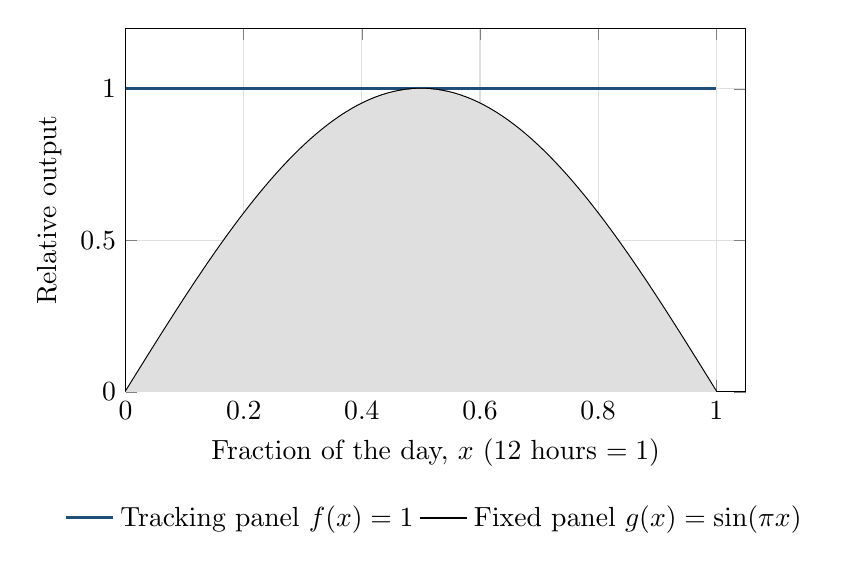
\begin{tikzpicture}
    \begin{axis}[
      width=0.78\textwidth, height=6.2cm,
      xlabel={Fraction of the day, $x$ (12 hours $=1$)},
      ylabel={Relative output},
      xmin=0, xmax=1.05, ymin=0, ymax=1.2,
      grid=both, grid style={gray!25},
      legend style={at={(0.5,-0.28)},anchor=north,draw=none},
      legend columns=2, legend cell align=left,
    ]
      \addplot[accent, very thick, domain=0:1] {1};
      \addplot[black, thick, domain=0:1, samples=100] {sin(deg(pi*x))};
      \addplot[black, draw=none, fill=gray!25, domain=0:1, samples=100] {sin(deg(pi*x))} \closedcycle;
      \legend{Tracking panel $f(x)=1$, Fixed panel $g(x)=\sin(\pi x)$}
    \end{axis}
  \end{tikzpicture}
  \caption{Relative output of a tracking panel and a fixed flat panel over one day in the idealised model. The tracking curve encloses an area of 1, the fixed curve (shaded) an area of $2/\pi\approx0.64$.}
  \label{fig:curves}
\end{figure}

\subsection{Estimated annual energy per square metre}
Shanghai received about \SI{2134.7}{\hour} of sunshine in 2022 according to CEIC data \cite{ceic}. Applying the standard estimate for panel output \cite{yes}, namely area $\times$ \SI{1000}{\watt\per\meter\squared} $\times$ efficiency $\times$ sun hours $\div\,1000$, the original calculation gives
\begin{equation}
  E_{\text{fixed}} \approx \SI{426.94}{\kilo\watt\hour\per\meter\squared}\text{ per year},
\end{equation}
which corresponds to a panel efficiency of \SI{20}{\percent}. Multiplying by $\pi/2$ gives
\begin{equation}
  E_{\text{tracking}} \approx \SI{670.64}{\kilo\watt\hour\per\meter\squared}\text{ per year},
\end{equation}
an increase of about \SI{243.70}{\kilo\watt\hour\per\meter\squared} per year.

\subsection{Limits of this estimate}
These figures are a theoretical upper bound and should be read with care. The model assumes the fixed panel lies flat, whereas real fixed panels are usually tilted toward the sun, which narrows the gap. It also treats every sunshine hour as full strength, and it assumes the sun's angle changes uniformly across the day. The \SI{57}{\percent} figure comes from calculation and was not measured with the prototype.

% ---------- 4 ----------
\section{Design and Construction}

\subsection{Hardware}
Figure~\ref{fig:proto} shows the prototype. The main components were:
\begin{itemize}[nosep]
  \item a frame cut from polypropylene sheets, joined with hot glue and nuts and bolts;
  \item two servo motors, one for each axis of rotation;
  \item an Arduino microcontroller that calculates the required movement;
  \item a solar panel with four LDRs that sense the light and send data to the Arduino;
  \item an LED that shows the power output of the panel, and a power switch.
\end{itemize}
We first sketched the outline of each frame piece on the polypropylene sheet and cut the pieces out, then assembled the prototype.

\begin{figure}[H]
  \centering
  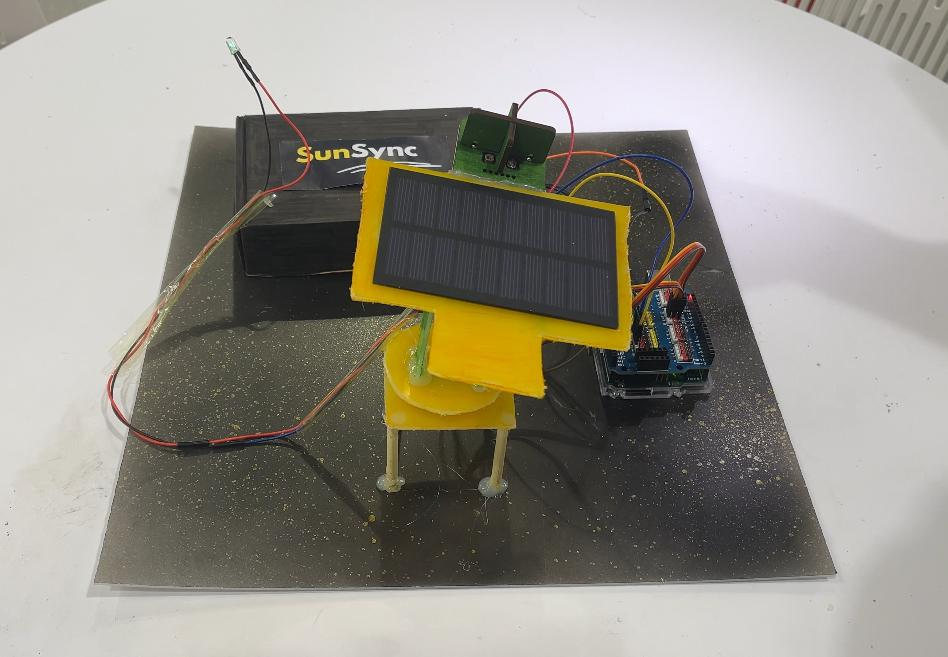
\includegraphics[width=0.7\textwidth]{../../images/prototype.jpg}
  \caption{The SunSync prototype: a solar panel on a two servo mount, with the Arduino board on the right and the LED power indicator on the left.}
  \label{fig:proto}
\end{figure}

\subsection{Control algorithm}
The Arduino sketch (\texttt{code/sun\_tracker/sun\_tracker.ino}) reads the four LDRs on analog pins A0 to A3 and compares light on opposite sides of the panel. With $V_{TL}$, $V_{TR}$, $V_{BL}$, $V_{BR}$ the readings from the top left, top right, bottom left and bottom right LDRs,
\begin{align}
  \Delta_{\text{vertical}}   &= (V_{TR}+V_{TL}) - (V_{BR}+V_{BL}),\\
  \Delta_{\text{horizontal}} &= (V_{TR}+V_{BR}) - (V_{TL}+V_{BL}).
\end{align}
For each axis, if the absolute difference exceeds a threshold of \num{50} ADC counts, the corresponding servo moves by one degree toward the brighter side. The sign of the difference sets the direction. The servo angles start at \ang{90} (centred) and are limited to \ang{0} to \ang{180}. The loop then waits \SI{80}{\milli\second}, so each axis can move at most about \SI{12.5}{\degree\per\second} (serial printing for debugging adds some delay in practice). Figure~\ref{fig:flow} summarises the loop.

\begin{figure}[H]
  \centering
  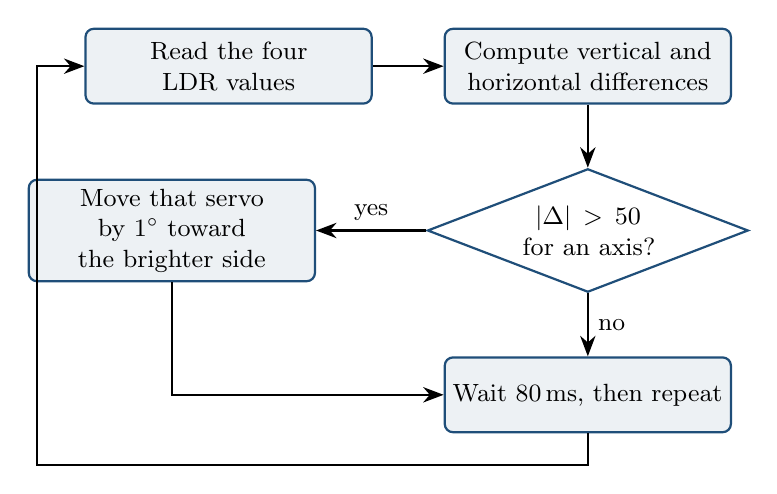
\begin{tikzpicture}[
    node distance=0.55cm and 0.9cm,
    box/.style={rectangle,rounded corners=3pt,draw=accent,fill=accent!8,thick,minimum height=0.95cm,text width=3.4cm,align=center,font=\small},
    dec/.style={diamond,aspect=2.6,draw=accent,fill=white,thick,text width=2.2cm,align=center,font=\small,inner sep=1pt},
    arr/.style={-{Stealth[length=2.6mm]},thick}
  ]
    \node[box] (read) {Read the four LDR values};
    \node[box,right=of read] (diff) {Compute vertical and horizontal differences};
    \node[dec,below=0.8cm of diff] (thr) {$|\Delta|>50$ for an axis?};
    \node[box,left=1.4cm of thr] (move) {Move that servo by \ang{1} toward the brighter side};
    \node[box,below=0.8cm of thr] (wait) {Wait \SI{80}{\milli\second}, then repeat};
    \draw[arr] (read) -- (diff);
    \draw[arr] (diff) -- (thr);
    \draw[arr] (thr) -- node[above,font=\small]{yes} (move);
    \draw[arr] (thr) -- node[right,font=\small]{no} (wait);
    \draw[arr] (move) |- (wait);
    \draw[arr] (wait.south) -- ++(0,-0.4) -| ($(read.west)+(-0.6,0)$) -- (read.west);
  \end{tikzpicture}
  \caption{Control loop of the tracker. The two axes are tested separately in every pass.}
  \label{fig:flow}
\end{figure}

% ---------- 5 ----------
\section{Experiments}

We ran two experiments on the prototype.

\textbf{Experiment 1: tracking a light source.} We switched the system on and shone a phone flashlight at the panel to check that it worked. We then moved the flashlight from one side to the other and watched whether the panel followed it. After that, we connected a power meter to the system and recorded the energy produced while the flashlight moved from one side to the centre, and the total energy produced while it moved from one side to the other. The experiment was run twice.

\textbf{Experiment 2: range of motion.} We checked how far the panel could rotate horizontally and vertically.

% ---------- 6 ----------
\section{Results}
\label{sec:results}

\begin{table}[H]
  \centering
  \caption{Result of Experiment 1: tracking of the flashlight.}
  \begin{tabular}{@{}ccc@{}}
    \toprule
    Trial & Panel tracks flashlight & Stable energy production \\
    \midrule
    1 & Yes & Yes \\
    2 & Yes & Yes \\
    \bottomrule
  \end{tabular}
\end{table}

In both trials the panel followed the flashlight and the energy production stayed stable. The exact power meter readings were not preserved, so no energy figures are reported here.

\begin{table}[H]
  \centering
  \caption{Result of Experiment 2: maximum turning angle per axis.}
  \begin{tabular}{@{}lc@{}}
    \toprule
    Direction & Maximum angle \\
    \midrule
    Horizontal & \ang{180} \\
    Vertical   & \ang{180} \\
    \bottomrule
  \end{tabular}
\end{table}

Both servos are commanded over \ang{0} to \ang{180} in the firmware, which matches Table~2.

% ---------- 7 ----------
\section{Discussion and Conclusion}
\label{sec:discussion}

The prototype met its main goal: the panel followed a moving light source on two axes, using only four LDRs and a simple comparison of their readings, and it produced a stable output while doing so.

The headline figure of the original report, \SI{57}{\percent} more energy, is different in kind. It comes from the idealised model in Section~\ref{sec:theory} and not from a measurement. The experiments showed that tracking works. They did not measure how much extra energy tracking gives compared with a fixed panel. Closing that gap is the most valuable next step: put a tracking panel and an identical fixed panel under the same light and log their output with the same meter over the same period.

% ---------- 8 ----------
\section{Outlook}

\subsection{Improvements}
\begin{itemize}[nosep]
  \item \textbf{Material.} The polypropylene frame is not durable enough to stay outdoors in sun and weather. Acrylic sheets, ABS plastic or aluminium would last longer.
  \item \textbf{Protection.} The cables and the Arduino should sit in a safer place, ideally a waterproof enclosure, to shield them from rain, dust and heat.
  \item \textbf{Servos.} Better quality servos, such as waterproof models, would give smoother turning and higher reliability.
\end{itemize}

\subsection{Future work}
\begin{itemize}[nosep]
  \item Measure tracking against a fixed panel under identical conditions, as described above.
  \item Test the panel outdoors in different weather, including rain and cloud.
  \item Scale the model up toward real applications.
  \item Study the lifetime of the motors by testing the strain caused by turning the panel.
\end{itemize}

% ---------- References ----------
\begin{thebibliography}{9}\small
  \bibitem{ipcc} IPCC. \emph{Climate Change in Data: The Physical Science Basis.} 2021. \url{https://www.ipcc.ch/report/ar6/wg1/resources/climate-change-in-data/}. Accessed 14 Dec 2024.
  \bibitem{cnet} CNET. ``Most Efficient Solar Panels for 2024: US Customers Still Waiting on Record-Setting Panel.'' 2024. \url{https://www.cnet.com/home/energy-and-utilities/most-efficient-solar-panels/}. Accessed 14 Dec 2024.
  \bibitem{helio} Barrette, J.J. ``What Is Heliotropism?'' West Virginia University Extension, June 2021. \url{https://extension.wvu.edu/lawn-gardening-pests/news/2021/06/01/what-is-heliotropism}. Accessed 14 Dec 2024.
  \bibitem{pv} ``Photovoltaic effect.'' \emph{Wikipedia}. \url{https://en.wikipedia.org/wiki/Photovoltaic_effect}. Accessed 14 Dec 2024.
  \bibitem{ceic} CEIC Data. China, sunshine hours (monthly, Shanghai, 2022). \url{https://www.ceicdata.com/}. Accessed 14 Dec 2024.
  \bibitem{yes} Yes Energy Solutions. ``How Much Energy Do Solar Panels Produce for a Home?'' \url{https://www.yesenergysolutions.co.uk/advice/how-much-energy-solar-panels-produce-home}. Accessed 14 Dec 2024.
\end{thebibliography}

\end{document}
